% Build me with pdflatex, then use pdf2svg to convert me to an svg file that can go into the repo!

\documentclass[crop, tikz]{standalone}

\usepackage[utf8]{inputenc}

\usetikzlibrary{shapes.arrows}

\newcommand{\arrow}[2]{
    \node[single arrow, draw=blue!50!black, very thick, fill=blue!50, minimum width=0.625cm, single arrow head extend=3pt, minimum height=#1 cm, rotate=#2] {};
}

\newcommand{\cellgrid}[1]{
    % Grid background
    \begin{scope}
        \draw[ultra thick, black, fill=black!20] (0,0) rectangle ({#1});
        \draw[step=1., black, thick] (0,0) grid ({#1});
    \end{scope}
}

\newcommand{\countrylabels}[1]{
    % Country labels at 0.5 height, with spacing 1
    \begin{scope}
        \foreach \i in {0, ..., #1}
            \node[anchor=east] at (0, #1 - \i + 0.5) {Country $\i$};
    \end{scope}
}

\newcommand{\datelabels}[2]{
    \begin{scope}
        \foreach \i in {0, ..., {#1}}
            \node[anchor=south] at (\i + 0.5, {#2}) {$\the\numexpr1952+\i*5 $};
    \end{scope}
}

\newcommand{\elipsis}[1]{
    \begin{scope}[shift={(0, 0.25)}]
        \foreach \i in {0, ..., 2}
            \filldraw[#1] (0,\i * 0.25) circle (1pt);
    \end{scope}
}

\newcommand{\dataframe}{
    \begin{scope}
        % Dataframe representation
        \begin{scope}[shift={(0,-1)}]
            % Dataframe and date labels
            \cellgrid{4, 5};
            \datelabels{2}{5};
            \begin{scope}[shift={(4,5.25)}]
                \begin{scope}[rotate=90]
                    \elipsis{black};
                \end{scope}
            \end{scope}
        \end{scope}
        % Row labels
        \countrylabels{3};
        \begin{scope}[shift={(-1,-1)}]
            \elipsis{black};
        \end{scope}
    \end{scope}
}

\begin{document}

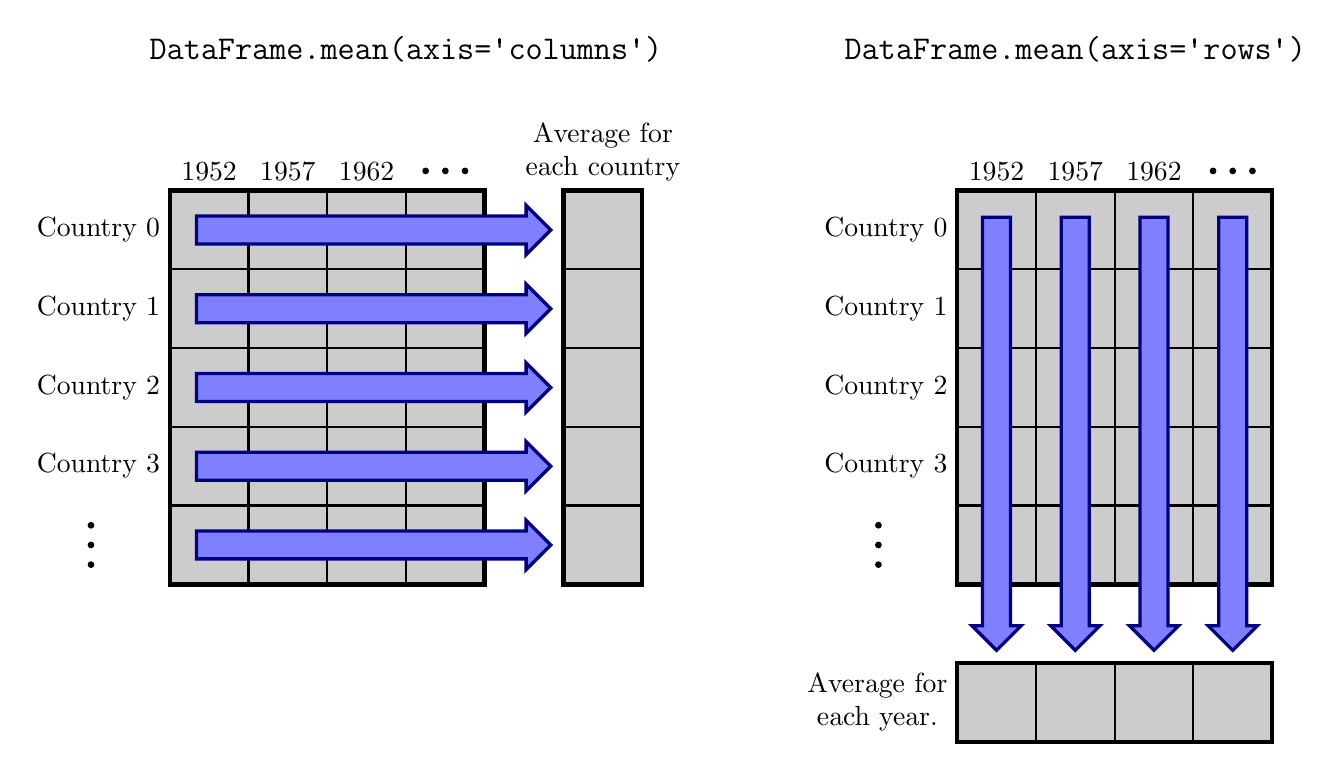
\begin{tikzpicture}

    % Operation across the columns (axis='columns')
    \begin{scope}[shift={(0,0)}]
        \dataframe;
        % Arrows across dataframe
        \foreach \i in {0, ..., 4} {
                \begin{scope}[shift={(2.5,\i-0.5)}]
                    \arrow{4.5}{0};
                \end{scope}
            }
        \begin{scope}[shift={(5,-1)}]
            \cellgrid{1, 5};
        \end{scope}

        % Label for resulting column dataframe
        \node[anchor=south, align=center] at (5.5,4) {Average for \\ each country};

        % Title above sub-diagram
        \node[anchor=south, align=center] at (3,5.5) {{\tt\large DataFrame.mean(axis=\textquotesingle{columns}\textquotesingle)}};
    \end{scope}

    % Operation across the rows (axis='rows')
    \begin{scope}[shift={(10,0)}]
        \dataframe;

        \begin{scope}[shift={(0,-3)}]
            \cellgrid{4, 1};
        \end{scope}

        \foreach \i in {0, ..., 3} {
                \begin{scope}[shift={(\i+0.5,1)}]
                    \arrow{5.5}{-90};
                \end{scope}
            }

        % Label for resulting row dataframe
        \node[anchor=east, align=center] at (0,-2.5) {Average for \\ each year.};

        % Title for sub-diagram
        \node[anchor=south, align=center] at (1.5,5.5) {{\tt\large DataFrame.mean(axis=\textquotesingle{rows}\textquotesingle)}};
    \end{scope}
\end{tikzpicture}

\end{document}